\subsubsection{Overview}
\label{Hodgkin-Huxley Neuron}
\index{Hodgkin-Huxley Neuron}\index{utilities, Hodkin-Huxley Neuron}
\begin{figure}[h]
\begin{center}
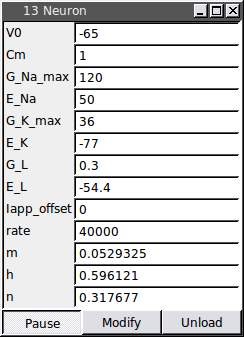
\includegraphics[width=2in]{hhneuron.png} 
\caption[HH Neuron]{GUI for a real-time Hodgkin-Huxley neuron within RTXI.} 
\end{center}
\label{hhneuron}
\end{figure}

This module contains the classic Hodgkin-Huxley model neuron. 

\subsubsection{Input Channels}
\begin{description}
\item[input(0)- Iapp] applied current (A)
\end{description}

\subsubsection{Output Channels}
\begin{description}
\item[output(0) - Vm] membrane voltage (V)
\end{description}

\subsubsection{Parameters}
\begin{description}
\item[V0] voltage (mV)
\item[Cm] membrane capacitance (uF/cm\^2)
\item[G\_Na\_max] max. Na+ conductance density  (mS/cm\^2)
\item[E\_Na] Na+ reversal potential (mV)
\item[G\_K\_max] max. K+ conductance density (mS/cm\^2)
\item[E\_K] K+ reversal potential (mV)
\item[G\_L] leak channel conductance density (mS/cm\^2)
\item[E\_L] leak channel reversal potential (mV)
\item[Iapp\_offset] offset current added to input (uA/cm\^2)
\item[rate] rate of integration (Hz)
\end{description}

\subsubsection{States}
\begin{description}
\item[m] sodium activation
\item[h] sodium inactivation
\item[n] potassium inactivation
\end{description}